% Created by tikzDevice version 0.7.0 on 2014-12-04 16:42:15
% !TEX encoding = UTF-8 Unicode
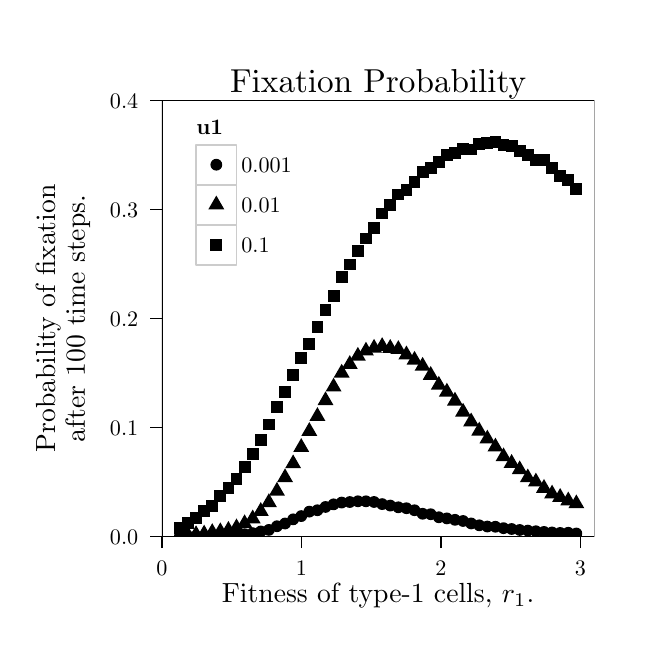
\begin{tikzpicture}[x=1pt,y=1pt]
\definecolor[named]{fillColor}{rgb}{1.00,1.00,1.00}
\path[use as bounding box,fill=fillColor,fill opacity=0.00] (0,0) rectangle (216.81,216.81);
\begin{scope}
\path[clip] (  0.00,  0.00) rectangle (216.81,216.81);
\definecolor[named]{drawColor}{rgb}{1.00,1.00,1.00}
\definecolor[named]{fillColor}{rgb}{1.00,1.00,1.00}

\path[draw=drawColor,line width= 0.6pt,line join=round,line cap=round,fill=fillColor] ( -0.00,  0.00) rectangle (216.81,216.81);
\end{scope}
\begin{scope}
\path[clip] ( 48.49, 32.98) rectangle (204.76,190.48);
\definecolor[named]{fillColor}{rgb}{1.00,1.00,1.00}

\path[fill=fillColor] ( 48.49, 32.98) rectangle (204.76,190.48);
\definecolor[named]{fillColor}{rgb}{0.00,0.00,0.00}

\path[fill=fillColor] ( 52.86, 33.85) --
	( 57.12, 33.85) --
	( 57.12, 38.12) --
	( 52.86, 38.12) --
	cycle;

\path[fill=fillColor] ( 55.78, 35.77) --
	( 60.05, 35.77) --
	( 60.05, 40.04) --
	( 55.78, 40.04) --
	cycle;

\path[fill=fillColor] ( 58.70, 37.44) --
	( 62.97, 37.44) --
	( 62.97, 41.70) --
	( 58.70, 41.70) --
	cycle;

\path[fill=fillColor] ( 61.63, 39.92) --
	( 65.90, 39.92) --
	( 65.90, 44.19) --
	( 61.63, 44.19) --
	cycle;

\path[fill=fillColor] ( 64.55, 41.97) --
	( 68.82, 41.97) --
	( 68.82, 46.24) --
	( 64.55, 46.24) --
	cycle;

\path[fill=fillColor] ( 67.48, 45.57) --
	( 71.74, 45.57) --
	( 71.74, 49.83) --
	( 67.48, 49.83) --
	cycle;

\path[fill=fillColor] ( 70.40, 48.32) --
	( 74.67, 48.32) --
	( 74.67, 52.59) --
	( 70.40, 52.59) --
	cycle;

\path[fill=fillColor] ( 73.32, 51.66) --
	( 77.59, 51.66) --
	( 77.59, 55.93) --
	( 73.32, 55.93) --
	cycle;

\path[fill=fillColor] ( 76.25, 56.07) --
	( 80.52, 56.07) --
	( 80.52, 60.34) --
	( 76.25, 60.34) --
	cycle;

\path[fill=fillColor] ( 79.17, 60.52) --
	( 83.44, 60.52) --
	( 83.44, 64.79) --
	( 79.17, 64.79) --
	cycle;

\path[fill=fillColor] ( 82.10, 65.70) --
	( 86.36, 65.70) --
	( 86.36, 69.97) --
	( 82.10, 69.97) --
	cycle;

\path[fill=fillColor] ( 85.02, 71.31) --
	( 89.29, 71.31) --
	( 89.29, 75.57) --
	( 85.02, 75.57) --
	cycle;

\path[fill=fillColor] ( 87.94, 77.50) --
	( 92.21, 77.50) --
	( 92.21, 81.76) --
	( 87.94, 81.76) --
	cycle;

\path[fill=fillColor] ( 90.87, 82.96) --
	( 95.14, 82.96) --
	( 95.14, 87.23) --
	( 90.87, 87.23) --
	cycle;

\path[fill=fillColor] ( 93.79, 89.20) --
	( 98.06, 89.20) --
	( 98.06, 93.47) --
	( 93.79, 93.47) --
	cycle;

\path[fill=fillColor] ( 96.72, 95.38) --
	(100.98, 95.38) --
	(100.98, 99.64) --
	( 96.72, 99.64) --
	cycle;

\path[fill=fillColor] ( 99.64,100.48) --
	(103.91,100.48) --
	(103.91,104.75) --
	( 99.64,104.75) --
	cycle;

\path[fill=fillColor] (102.56,106.55) --
	(106.83,106.55) --
	(106.83,110.82) --
	(102.56,110.82) --
	cycle;

\path[fill=fillColor] (105.49,112.75) --
	(109.76,112.75) --
	(109.76,117.02) --
	(105.49,117.02) --
	cycle;

\path[fill=fillColor] (108.41,117.68) --
	(112.68,117.68) --
	(112.68,121.95) --
	(108.41,121.95) --
	cycle;

\path[fill=fillColor] (111.33,124.56) --
	(115.60,124.56) --
	(115.60,128.82) --
	(111.33,128.82) --
	cycle;

\path[fill=fillColor] (114.26,129.10) --
	(118.53,129.10) --
	(118.53,133.37) --
	(114.26,133.37) --
	cycle;

\path[fill=fillColor] (117.18,134.11) --
	(121.45,134.11) --
	(121.45,138.38) --
	(117.18,138.38) --
	cycle;

\path[fill=fillColor] (120.11,138.52) --
	(124.37,138.52) --
	(124.37,142.79) --
	(120.11,142.79) --
	cycle;

\path[fill=fillColor] (123.03,142.38) --
	(127.30,142.38) --
	(127.30,146.65) --
	(123.03,146.65) --
	cycle;

\path[fill=fillColor] (125.95,147.54) --
	(130.22,147.54) --
	(130.22,151.81) --
	(125.95,151.81) --
	cycle;

\path[fill=fillColor] (128.88,150.65) --
	(133.15,150.65) --
	(133.15,154.91) --
	(128.88,154.91) --
	cycle;

\path[fill=fillColor] (131.80,154.38) --
	(136.07,154.38) --
	(136.07,158.64) --
	(131.80,158.64) --
	cycle;

\path[fill=fillColor] (134.73,155.93) --
	(138.99,155.93) --
	(138.99,160.20) --
	(134.73,160.20) --
	cycle;

\path[fill=fillColor] (137.65,159.01) --
	(141.92,159.01) --
	(141.92,163.27) --
	(137.65,163.27) --
	cycle;

\path[fill=fillColor] (140.57,162.64) --
	(144.84,162.64) --
	(144.84,166.91) --
	(140.57,166.91) --
	cycle;

\path[fill=fillColor] (143.50,164.00) --
	(147.77,164.00) --
	(147.77,168.27) --
	(143.50,168.27) --
	cycle;

\path[fill=fillColor] (146.42,166.09) --
	(150.69,166.09) --
	(150.69,170.36) --
	(146.42,170.36) --
	cycle;

\path[fill=fillColor] (149.35,168.63) --
	(153.61,168.63) --
	(153.61,172.90) --
	(149.35,172.90) --
	cycle;

\path[fill=fillColor] (152.27,169.41) --
	(156.54,169.41) --
	(156.54,173.68) --
	(152.27,173.68) --
	cycle;

\path[fill=fillColor] (155.19,170.69) --
	(159.46,170.69) --
	(159.46,174.96) --
	(155.19,174.96) --
	cycle;

\path[fill=fillColor] (158.12,170.64) --
	(162.39,170.64) --
	(162.39,174.91) --
	(158.12,174.91) --
	cycle;

\path[fill=fillColor] (161.04,172.51) --
	(165.31,172.51) --
	(165.31,176.78) --
	(161.04,176.78) --
	cycle;

\path[fill=fillColor] (163.97,172.87) --
	(168.23,172.87) --
	(168.23,177.14) --
	(163.97,177.14) --
	cycle;

\path[fill=fillColor] (166.89,173.31) --
	(171.16,173.31) --
	(171.16,177.58) --
	(166.89,177.58) --
	cycle;

\path[fill=fillColor] (169.81,172.41) --
	(174.08,172.41) --
	(174.08,176.68) --
	(169.81,176.68) --
	cycle;

\path[fill=fillColor] (172.74,171.82) --
	(177.00,171.82) --
	(177.00,176.09) --
	(172.74,176.09) --
	cycle;

\path[fill=fillColor] (175.66,170.01) --
	(179.93,170.01) --
	(179.93,174.28) --
	(175.66,174.28) --
	cycle;

\path[fill=fillColor] (178.58,168.78) --
	(182.85,168.78) --
	(182.85,173.05) --
	(178.58,173.05) --
	cycle;

\path[fill=fillColor] (181.51,166.80) --
	(185.78,166.80) --
	(185.78,171.07) --
	(181.51,171.07) --
	cycle;

\path[fill=fillColor] (184.43,166.86) --
	(188.70,166.86) --
	(188.70,171.12) --
	(184.43,171.12) --
	cycle;

\path[fill=fillColor] (187.36,164.11) --
	(191.62,164.11) --
	(191.62,168.38) --
	(187.36,168.38) --
	cycle;

\path[fill=fillColor] (190.28,161.04) --
	(194.55,161.04) --
	(194.55,165.31) --
	(190.28,165.31) --
	cycle;

\path[fill=fillColor] (193.20,159.71) --
	(197.47,159.71) --
	(197.47,163.98) --
	(193.20,163.98) --
	cycle;

\path[fill=fillColor] (196.13,156.23) --
	(200.40,156.23) --
	(200.40,160.50) --
	(196.13,160.50) --
	cycle;

\path[fill=fillColor] ( 54.99, 36.59) --
	( 57.86, 31.61) --
	( 52.12, 31.61) --
	cycle;

\path[fill=fillColor] ( 57.91, 36.78) --
	( 60.79, 31.81) --
	( 55.04, 31.81) --
	cycle;

\path[fill=fillColor] ( 60.84, 37.00) --
	( 63.71, 32.02) --
	( 57.96, 32.02) --
	cycle;

\path[fill=fillColor] ( 63.76, 37.22) --
	( 66.64, 32.24) --
	( 60.89, 32.24) --
	cycle;

\path[fill=fillColor] ( 66.69, 37.75) --
	( 69.56, 32.78) --
	( 63.81, 32.78) --
	cycle;

\path[fill=fillColor] ( 69.61, 38.05) --
	( 72.48, 33.07) --
	( 66.74, 33.07) --
	cycle;

\path[fill=fillColor] ( 72.53, 38.55) --
	( 75.41, 33.57) --
	( 69.66, 33.57) --
	cycle;

\path[fill=fillColor] ( 75.46, 39.46) --
	( 78.33, 34.48) --
	( 72.58, 34.48) --
	cycle;

\path[fill=fillColor] ( 78.38, 40.95) --
	( 81.26, 35.97) --
	( 75.51, 35.97) --
	cycle;

\path[fill=fillColor] ( 81.31, 42.70) --
	( 84.18, 37.72) --
	( 78.43, 37.72) --
	cycle;

\path[fill=fillColor] ( 84.23, 45.38) --
	( 87.10, 40.41) --
	( 81.36, 40.41) --
	cycle;

\path[fill=fillColor] ( 87.15, 48.58) --
	( 90.03, 43.60) --
	( 84.28, 43.60) --
	cycle;

\path[fill=fillColor] ( 90.08, 52.69) --
	( 92.95, 47.71) --
	( 87.20, 47.71) --
	cycle;

\path[fill=fillColor] ( 93.00, 57.57) --
	( 95.88, 52.59) --
	( 90.13, 52.59) --
	cycle;

\path[fill=fillColor] ( 95.93, 62.60) --
	( 98.80, 57.62) --
	( 93.05, 57.62) --
	cycle;

\path[fill=fillColor] ( 98.85, 68.51) --
	(101.72, 63.53) --
	( 95.98, 63.53) --
	cycle;

\path[fill=fillColor] (101.77, 74.29) --
	(104.65, 69.31) --
	( 98.90, 69.31) --
	cycle;

\path[fill=fillColor] (104.70, 79.70) --
	(107.57, 74.73) --
	(101.82, 74.73) --
	cycle;

\path[fill=fillColor] (107.62, 85.40) --
	(110.50, 80.42) --
	(104.75, 80.42) --
	cycle;

\path[fill=fillColor] (110.54, 90.33) --
	(113.42, 85.35) --
	(107.67, 85.35) --
	cycle;

\path[fill=fillColor] (113.47, 95.35) --
	(116.34, 90.37) --
	(110.59, 90.37) --
	cycle;

\path[fill=fillColor] (116.39, 98.49) --
	(119.27, 93.52) --
	(113.52, 93.52) --
	cycle;

\path[fill=fillColor] (119.32,101.46) --
	(122.19, 96.48) --
	(116.44, 96.48) --
	cycle;

\path[fill=fillColor] (122.24,103.32) --
	(125.11, 98.35) --
	(119.37, 98.35) --
	cycle;

\path[fill=fillColor] (125.16,104.36) --
	(128.04, 99.38) --
	(122.29, 99.38) --
	cycle;

\path[fill=fillColor] (128.09,104.97) --
	(130.96,100.00) --
	(125.21,100.00) --
	cycle;

\path[fill=fillColor] (131.01,104.31) --
	(133.89, 99.33) --
	(128.14, 99.33) --
	cycle;

\path[fill=fillColor] (133.94,103.90) --
	(136.81, 98.92) --
	(131.06, 98.92) --
	cycle;

\path[fill=fillColor] (136.86,101.97) --
	(139.73, 96.99) --
	(133.99, 96.99) --
	cycle;

\path[fill=fillColor] (139.78,100.03) --
	(142.66, 95.05) --
	(136.91, 95.05) --
	cycle;

\path[fill=fillColor] (142.71, 97.85) --
	(145.58, 92.87) --
	(139.83, 92.87) --
	cycle;

\path[fill=fillColor] (145.63, 94.56) --
	(148.51, 89.58) --
	(142.76, 89.58) --
	cycle;

\path[fill=fillColor] (148.56, 91.00) --
	(151.43, 86.02) --
	(145.68, 86.02) --
	cycle;

\path[fill=fillColor] (151.48, 88.51) --
	(154.35, 83.53) --
	(148.61, 83.53) --
	cycle;

\path[fill=fillColor] (154.40, 85.26) --
	(157.28, 80.28) --
	(151.53, 80.28) --
	cycle;

\path[fill=fillColor] (157.33, 81.26) --
	(160.20, 76.28) --
	(154.45, 76.28) --
	cycle;

\path[fill=fillColor] (160.25, 77.75) --
	(163.13, 72.77) --
	(157.38, 72.77) --
	cycle;

\path[fill=fillColor] (163.18, 74.42) --
	(166.05, 69.44) --
	(160.30, 69.44) --
	cycle;

\path[fill=fillColor] (166.10, 71.54) --
	(168.97, 66.57) --
	(163.23, 66.57) --
	cycle;

\path[fill=fillColor] (169.02, 68.65) --
	(171.90, 63.67) --
	(166.15, 63.67) --
	cycle;

\path[fill=fillColor] (171.95, 65.13) --
	(174.82, 60.16) --
	(169.07, 60.16) --
	cycle;

\path[fill=fillColor] (174.87, 62.75) --
	(177.74, 57.77) --
	(172.00, 57.77) --
	cycle;

\path[fill=fillColor] (177.79, 60.44) --
	(180.67, 55.46) --
	(174.92, 55.46) --
	cycle;

\path[fill=fillColor] (180.72, 57.52) --
	(183.59, 52.55) --
	(177.84, 52.55) --
	cycle;

\path[fill=fillColor] (183.64, 56.02) --
	(186.52, 51.04) --
	(180.77, 51.04) --
	cycle;

\path[fill=fillColor] (186.57, 53.73) --
	(189.44, 48.75) --
	(183.69, 48.75) --
	cycle;

\path[fill=fillColor] (189.49, 51.68) --
	(192.36, 46.70) --
	(186.62, 46.70) --
	cycle;

\path[fill=fillColor] (192.41, 50.46) --
	(195.29, 45.49) --
	(189.54, 45.49) --
	cycle;

\path[fill=fillColor] (195.34, 49.20) --
	(198.21, 44.22) --
	(192.46, 44.22) --
	cycle;

\path[fill=fillColor] (198.26, 48.14) --
	(201.14, 43.17) --
	(195.39, 43.17) --
	cycle;

\path[fill=fillColor] ( 54.99, 33.02) circle (  2.13);

\path[fill=fillColor] ( 57.91, 33.04) circle (  2.13);

\path[fill=fillColor] ( 60.84, 33.07) circle (  2.13);

\path[fill=fillColor] ( 63.76, 33.08) circle (  2.13);

\path[fill=fillColor] ( 66.69, 33.10) circle (  2.13);

\path[fill=fillColor] ( 69.61, 33.19) circle (  2.13);

\path[fill=fillColor] ( 72.53, 33.27) circle (  2.13);

\path[fill=fillColor] ( 75.46, 33.46) circle (  2.13);

\path[fill=fillColor] ( 78.38, 33.76) circle (  2.13);

\path[fill=fillColor] ( 81.31, 34.16) circle (  2.13);

\path[fill=fillColor] ( 84.23, 34.77) circle (  2.13);

\path[fill=fillColor] ( 87.15, 35.33) circle (  2.13);

\path[fill=fillColor] ( 90.08, 36.65) circle (  2.13);

\path[fill=fillColor] ( 93.00, 37.64) circle (  2.13);

\path[fill=fillColor] ( 95.93, 39.14) circle (  2.13);

\path[fill=fillColor] ( 98.85, 40.32) circle (  2.13);

\path[fill=fillColor] (101.77, 41.93) circle (  2.13);

\path[fill=fillColor] (104.70, 42.43) circle (  2.13);

\path[fill=fillColor] (107.62, 43.62) circle (  2.13);

\path[fill=fillColor] (110.54, 44.56) circle (  2.13);

\path[fill=fillColor] (113.47, 45.21) circle (  2.13);

\path[fill=fillColor] (116.39, 45.40) circle (  2.13);

\path[fill=fillColor] (119.32, 45.67) circle (  2.13);

\path[fill=fillColor] (122.24, 45.66) circle (  2.13);

\path[fill=fillColor] (125.16, 45.42) circle (  2.13);

\path[fill=fillColor] (128.09, 44.65) circle (  2.13);

\path[fill=fillColor] (131.01, 44.12) circle (  2.13);

\path[fill=fillColor] (133.94, 43.50) circle (  2.13);

\path[fill=fillColor] (136.86, 43.16) circle (  2.13);

\path[fill=fillColor] (139.78, 42.43) circle (  2.13);

\path[fill=fillColor] (142.71, 41.16) circle (  2.13);

\path[fill=fillColor] (145.63, 40.99) circle (  2.13);

\path[fill=fillColor] (148.56, 39.90) circle (  2.13);

\path[fill=fillColor] (151.48, 39.49) circle (  2.13);

\path[fill=fillColor] (154.40, 38.97) circle (  2.13);

\path[fill=fillColor] (157.33, 38.55) circle (  2.13);

\path[fill=fillColor] (160.25, 37.66) circle (  2.13);

\path[fill=fillColor] (163.18, 36.99) circle (  2.13);

\path[fill=fillColor] (166.10, 36.55) circle (  2.13);

\path[fill=fillColor] (169.02, 36.47) circle (  2.13);

\path[fill=fillColor] (171.95, 35.95) circle (  2.13);

\path[fill=fillColor] (174.87, 35.65) circle (  2.13);

\path[fill=fillColor] (177.79, 35.30) circle (  2.13);

\path[fill=fillColor] (180.72, 35.08) circle (  2.13);

\path[fill=fillColor] (183.64, 34.84) circle (  2.13);

\path[fill=fillColor] (186.57, 34.60) circle (  2.13);

\path[fill=fillColor] (189.49, 34.40) circle (  2.13);

\path[fill=fillColor] (192.41, 34.23) circle (  2.13);

\path[fill=fillColor] (195.34, 34.30) circle (  2.13);

\path[fill=fillColor] (198.26, 34.03) circle (  2.13);
\definecolor[named]{drawColor}{rgb}{0.00,0.00,0.00}

\path[draw=drawColor,line width= 0.6pt,line join=round,line cap=round] ( 48.49, 32.98) rectangle (204.76,190.48);
\end{scope}
\begin{scope}
\path[clip] (  0.00,  0.00) rectangle (216.81,216.81);
\definecolor[named]{drawColor}{rgb}{0.00,0.00,0.00}

\node[text=drawColor,anchor=base east,inner sep=0pt, outer sep=0pt, scale=  0.80] at ( 39.95, 30.22) {0.0};

\node[text=drawColor,anchor=base east,inner sep=0pt, outer sep=0pt, scale=  0.80] at ( 39.95, 69.60) {0.1};

\node[text=drawColor,anchor=base east,inner sep=0pt, outer sep=0pt, scale=  0.80] at ( 39.95,108.97) {0.2};

\node[text=drawColor,anchor=base east,inner sep=0pt, outer sep=0pt, scale=  0.80] at ( 39.95,148.35) {0.3};

\node[text=drawColor,anchor=base east,inner sep=0pt, outer sep=0pt, scale=  0.80] at ( 39.95,187.72) {0.4};
\end{scope}
\begin{scope}
\path[clip] (  0.00,  0.00) rectangle (216.81,216.81);
\definecolor[named]{drawColor}{rgb}{0.00,0.00,0.00}

\path[draw=drawColor,line width= 0.6pt,line join=round] ( 44.22, 32.98) --
	( 48.49, 32.98);

\path[draw=drawColor,line width= 0.6pt,line join=round] ( 44.22, 72.35) --
	( 48.49, 72.35);

\path[draw=drawColor,line width= 0.6pt,line join=round] ( 44.22,111.73) --
	( 48.49,111.73);

\path[draw=drawColor,line width= 0.6pt,line join=round] ( 44.22,151.10) --
	( 48.49,151.10);

\path[draw=drawColor,line width= 0.6pt,line join=round] ( 44.22,190.48) --
	( 48.49,190.48);
\end{scope}
\begin{scope}
\path[clip] (  0.00,  0.00) rectangle (216.81,216.81);
\definecolor[named]{drawColor}{rgb}{0.00,0.00,0.00}

\path[draw=drawColor,line width= 0.6pt,line join=round] ( 48.49, 28.71) --
	( 48.49, 32.98);

\path[draw=drawColor,line width= 0.6pt,line join=round] ( 98.90, 28.71) --
	( 98.90, 32.98);

\path[draw=drawColor,line width= 0.6pt,line join=round] (149.31, 28.71) --
	(149.31, 32.98);

\path[draw=drawColor,line width= 0.6pt,line join=round] (199.72, 28.71) --
	(199.72, 32.98);
\end{scope}
\begin{scope}
\path[clip] (  0.00,  0.00) rectangle (216.81,216.81);
\definecolor[named]{drawColor}{rgb}{0.00,0.00,0.00}

\node[text=drawColor,anchor=base,inner sep=0pt, outer sep=0pt, scale=  0.80] at ( 48.49, 18.93) {0};

\node[text=drawColor,anchor=base,inner sep=0pt, outer sep=0pt, scale=  0.80] at ( 98.90, 18.93) {1};

\node[text=drawColor,anchor=base,inner sep=0pt, outer sep=0pt, scale=  0.80] at (149.31, 18.93) {2};

\node[text=drawColor,anchor=base,inner sep=0pt, outer sep=0pt, scale=  0.80] at (199.72, 18.93) {3};
\end{scope}
\begin{scope}
\path[clip] (  0.00,  0.00) rectangle (216.81,216.81);
\definecolor[named]{drawColor}{rgb}{0.00,0.00,0.00}

\node[text=drawColor,anchor=base,inner sep=0pt, outer sep=0pt, scale=  1.00] at (126.63,  9.03) {Fitness of type-1 cells, $r_1$.};
\end{scope}
\begin{scope}
\path[clip] (  0.00,  0.00) rectangle (216.81,216.81);
\definecolor[named]{drawColor}{rgb}{0.00,0.00,0.00}

\node[text=drawColor,rotate= 90.00,anchor=base,inner sep=0pt, outer sep=0pt, scale=  1.00] at (  9.90,111.73) {Probability of fixation };

\node[text=drawColor,rotate= 90.00,anchor=base,inner sep=0pt, outer sep=0pt, scale=  1.00] at ( 20.70,111.73) {  after 100 time steps.};
\end{scope}
\begin{scope}
\path[clip] (  0.00,  0.00) rectangle (216.81,216.81);
\definecolor[named]{fillColor}{rgb}{1.00,1.00,1.00}

\path[fill=fillColor] ( 56.67,126.89) rectangle ( 99.69,187.92);
\end{scope}
\begin{scope}
\path[clip] (  0.00,  0.00) rectangle (216.81,216.81);
\definecolor[named]{drawColor}{rgb}{0.00,0.00,0.00}

\node[text=drawColor,anchor=base west,inner sep=0pt, outer sep=0pt, scale=  0.80] at ( 60.94,178.13) {\bfseries u1};
\end{scope}
\begin{scope}
\path[clip] (  0.00,  0.00) rectangle (216.81,216.81);
\definecolor[named]{drawColor}{rgb}{0.80,0.80,0.80}
\definecolor[named]{fillColor}{rgb}{1.00,1.00,1.00}

\path[draw=drawColor,line width= 0.6pt,line join=round,line cap=round,fill=fillColor] ( 60.94,160.06) rectangle ( 75.40,174.52);
\end{scope}
\begin{scope}
\path[clip] (  0.00,  0.00) rectangle (216.81,216.81);
\definecolor[named]{fillColor}{rgb}{0.00,0.00,0.00}

\path[fill=fillColor] ( 68.17,167.29) circle (  2.13);
\end{scope}
\begin{scope}
\path[clip] (  0.00,  0.00) rectangle (216.81,216.81);
\definecolor[named]{drawColor}{rgb}{0.80,0.80,0.80}
\definecolor[named]{fillColor}{rgb}{1.00,1.00,1.00}

\path[draw=drawColor,line width= 0.6pt,line join=round,line cap=round,fill=fillColor] ( 60.94,145.61) rectangle ( 75.40,160.06);
\end{scope}
\begin{scope}
\path[clip] (  0.00,  0.00) rectangle (216.81,216.81);
\definecolor[named]{fillColor}{rgb}{0.00,0.00,0.00}

\path[fill=fillColor] ( 68.17,156.15) --
	( 71.04,151.18) --
	( 65.29,151.18) --
	cycle;
\end{scope}
\begin{scope}
\path[clip] (  0.00,  0.00) rectangle (216.81,216.81);
\definecolor[named]{drawColor}{rgb}{0.80,0.80,0.80}
\definecolor[named]{fillColor}{rgb}{1.00,1.00,1.00}

\path[draw=drawColor,line width= 0.6pt,line join=round,line cap=round,fill=fillColor] ( 60.94,131.15) rectangle ( 75.40,145.61);
\end{scope}
\begin{scope}
\path[clip] (  0.00,  0.00) rectangle (216.81,216.81);
\definecolor[named]{fillColor}{rgb}{0.00,0.00,0.00}

\path[fill=fillColor] ( 66.03,136.25) --
	( 70.30,136.25) --
	( 70.30,140.52) --
	( 66.03,140.52) --
	cycle;
\end{scope}
\begin{scope}
\path[clip] (  0.00,  0.00) rectangle (216.81,216.81);
\definecolor[named]{drawColor}{rgb}{0.00,0.00,0.00}

\node[text=drawColor,anchor=base west,inner sep=0pt, outer sep=0pt, scale=  0.80] at ( 77.20,164.53) {0.001};
\end{scope}
\begin{scope}
\path[clip] (  0.00,  0.00) rectangle (216.81,216.81);
\definecolor[named]{drawColor}{rgb}{0.00,0.00,0.00}

\node[text=drawColor,anchor=base west,inner sep=0pt, outer sep=0pt, scale=  0.80] at ( 77.20,150.08) {0.01};
\end{scope}
\begin{scope}
\path[clip] (  0.00,  0.00) rectangle (216.81,216.81);
\definecolor[named]{drawColor}{rgb}{0.00,0.00,0.00}

\node[text=drawColor,anchor=base west,inner sep=0pt, outer sep=0pt, scale=  0.80] at ( 77.20,135.63) {0.1};
\end{scope}
\begin{scope}
\path[clip] (  0.00,  0.00) rectangle (216.81,216.81);
\definecolor[named]{drawColor}{rgb}{0.00,0.00,0.00}

\node[text=drawColor,anchor=base,inner sep=0pt, outer sep=0pt, scale=  1.20] at (126.63,193.49) {Fixation Probability};
\end{scope}
\end{tikzpicture}
